% A line bundle chart over the disk |z-3| < 2 (real part (1,5)).
% Source: book/tex/riemann-surface/line-bundles.tex (asy figure).
\documentclass[border=2mm]{standalone}
\usepackage{tikz}
\begin{document}
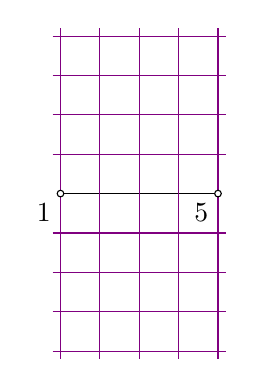
\begin{tikzpicture}[scale=0.5,>=latex]
  \draw (1,0) -- (5,0);
  \node[anchor=north east] at (1,0) {$1$};
  \node[anchor=north east] at (5,0) {$5$};
  \draw[violet] (1,-4.2) -- (1,4.2);
  \draw[violet] (2,-4.2) -- (2,4.2);
  \draw[violet] (3,-4.2) -- (3,4.2);
  \draw[violet] (4,-4.2) -- (4,4.2);
  \draw[violet] (5,-4.2) -- (5,4.2);
  \draw[violet] (0.8,-4) -- (5.2,-4);
  \draw[violet] (0.8,-3) -- (5.2,-3);
  \draw[violet] (0.8,-2) -- (5.2,-2);
  \draw[violet] (0.8,-1) -- (5.2,-1);
  \draw[violet] (0.8,1) -- (5.2,1);
  \draw[violet] (0.8,2) -- (5.2,2);
  \draw[violet] (0.8,3) -- (5.2,3);
  \draw[violet] (0.8,4) -- (5.2,4);
  \filldraw[fill=white] (1,0) circle (2.4pt);
  \filldraw[fill=white] (5,0) circle (2.4pt);
\end{tikzpicture}
\end{document}
